\documentclass[a4paper,12pt]{article}
\usepackage[utf8]{inputenc}
\usepackage[english]{babel}
\usepackage{blindtext}
\usepackage{authblk}
\usepackage{graphics}
\usepackage{graphicx}
\usepackage{mathptmx}
\usepackage[singlespacing]{setspace}
\usepackage[margin=1in]{geometry}
\graphicspath{{images/}}


\title{IC$^{2}$S$^{2}$ 2018 Submission: Insert Title Here \\
	\normalsize $4$$^{th}$ International Conference on Computational Social Science IC$^{2}$S$^{2}$ \\
	\normalsize July 12-15, 2018 \\
	\normalsize Northwestern University’s Kellogg School of Management \\
	\normalsize Evanston, IL. USA
}



\author[1]{Anonymous} % Please leave Author-field blank for blind review and remove information that may identify the author(s)
 
\date{}

\begin{document}

\maketitle

\vspace{-2em}

\begin{center}
\textbf{\textit{keywords: Uber, behavior and social aspects of health, Google Search, flu-like illness, Internet }}
\newline
\end{center}


\section{Extended Abstract}
Ride-hailing services, such as Uber and Lyft, are disrupting the transportation system worldwide having a pronounced impact on people's usage patterns. In 2016, Subway ridership in New York declined for the first time in years, whereas ride-hailing services became the leading source of growth in non-auto travel \cite{schaller2017unsustainable}. However, there are mixed results about the relationship between ride-hailing services and public transportation. For example, a Pew study suggests that ride-hailing is complementary to public transit and walking %\cite{smith2016shared}, while current evidence suggests that ride-hailing is pulling more people away from public transit in cities \cite{clewlow2017disruptive}. One thing is clear: ride-hailing is changing the way we move in cities. 

In this paper, we study the effects of ride-hailing on health related issues, particularly, the spread of flu-related illness. There is evidence suggesting that public transportation is important in the propagation of influenza-like illness in winter \cite{troko2011public,cooley2011role}. Based on these results, we hypothesize that a change in how people commute, as a consequence of ride-hailing services, can have an effect on the contagious levels of influenza in the population. Here, we present one of the first quantitative explorations of the relationship between ride-hailing services and health. We exploit the fact that UberX, the first and most popular ride-hailing platform, was rolled out across the US piecewise and not all at once (depicted in Figure \ref{fig:Uber} for a sample of cities). Thus, we are provided with an excellent natural experiment setting to identify its impact. 

Unfortunately, weekly US Influenza Surveillance reports are aggregated at a state level and to our knowledge there is no other source that provides finer granularity levels. However, we can rely on Google Flu Trends as a proxy to measure flu-related illness at a city level. Google Flu Trends utilizes internet search queries to detect the presence of influenza like illness and has been use effectively for Influenza forecasting \cite{yang2015accurate,dugas2013influenza}.

Similar to Berger et al's. paper \cite{berger2017drivers}, where Uber's impact on unemployment was studied, we use a difference-in-differences approach to compare changes in the influenza levels in U.S. cities before and after UberX and UberPool introduction. Our baseline regression model is
\[
y_{it}=city_{i}+year_{t}+month_{t}+\alpha Uber_{it}+\beta Pool_{it}+\gamma X_{it}+ \varepsilon_{it},
\]
where $y_{it}$ is flu estimate for city $i$ and month $t$; fixed effects variables $city_{i}$, $year_{t}$ and $month_{t}$ account, respectively, for time-invariant differences in city baseline levels, city-invariant US yearly pandemic levels, and the seasonality nature of flu. $Uber_{it}$ and $ Pool_{it}$ take the form of a dummy variable representing if UberX and UberPool services are present in city $i$ and month $t$; $X_{it}$ are time varying and city characteristics to control for weather data such as monthly min and max temperatures and monthly precipitation.







\bibliographystyle{plain}
\bibliography{references}

\section{Figure(s)}

\begin{figure}[htp]
\centering
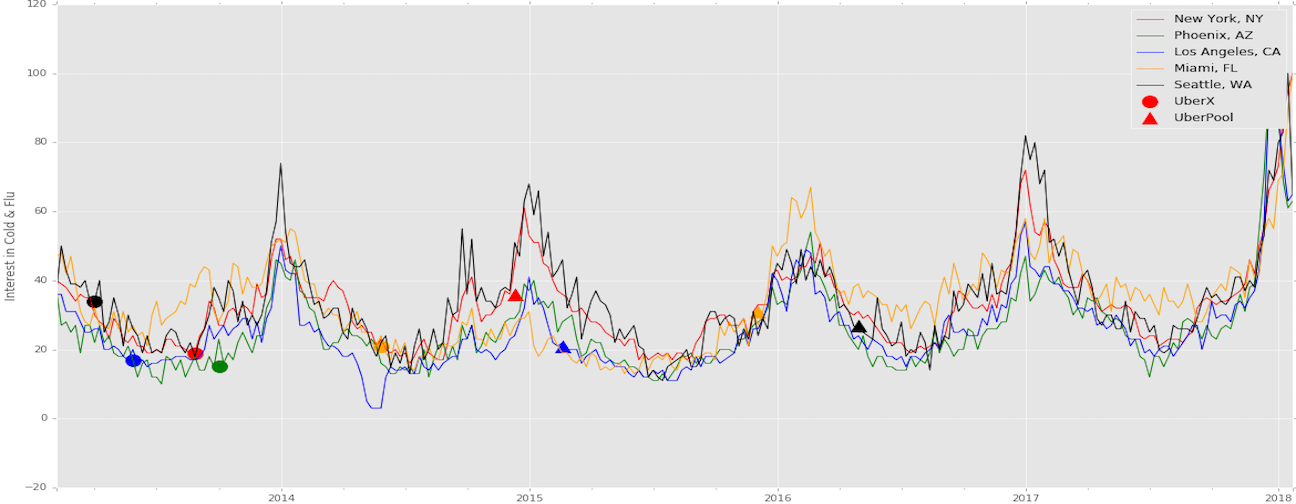
\includegraphics[width=13cm]{images/fig1}
\vspace{-0.5em}
\caption{Google monthly Flu trends over time for various cities. Circle and triangle marks identify the time when UberX and UberPool were introduced for each city, respectively.}
\label{fig:Uber}
\end{figure}


\end{document}
